\ifx\isEmbedded\undefined
\documentclass[12pt]{article}
	
% FONT RELATED
%\usepackage{times} %Move to times font
\usepackage[labelfont=bf,textfont=it]{caption}


% LINKS, PAGE OF CONTENT, REF AND CROSS-REF, HEADERS/FOOTERS
\usepackage{hyperref}
\hypersetup{
    colorlinks,
    citecolor=black,
    filecolor=black,
    linkcolor=black,
    urlcolor=black
}
%\usepackage[breaklinks=true]{hyperref}
\usepackage{fancyhdr}
\usepackage{acronym}

% FIGURES, GRAPHICS, TABLES
\usepackage{graphicx}
\usepackage{parskip}
\usepackage{subfigure}

% COLOURS, TEXT AND FORMATTING
\usepackage{array}
\usepackage{color}
\usepackage{setspace}
\usepackage{longtable}
\usepackage{multirow}

% ADVANCED MATHS, PSEUDO-CODE
\usepackage{amsmath}
\usepackage{alltt}
\usepackage{amsfonts}
\usepackage{listings}
\usepackage{amsmath}

% BIBLIOGRAPHY
\usepackage[authoryear]{natbib}
\bibpunct{(}{)}{;}{a}{}{,}

% USE IN DISSER:

\setlength\oddsidemargin{1.5cm}
\setlength\evensidemargin{5cm}

\setlength\textheight{9.0in}
\setlength\textwidth{5.1in}

% indent at each new paragrapg
\setlength\parindent{0.5cm}

\setlength\topmargin{-0.2in}
\renewcommand{\baselinestretch}{1.3}

%REPORT

%\setlength\oddsidemargin{1cm}
%\setlength\evensidemargin{0.3in}
%%\setlength\headsep{2.5in}
%
%\setlength\textheight{9.0in}
%\setlength\textwidth{5.5in}
%
%% indent at each new paragrapg
%\setlength\parindent{0.5cm}
%
%%\setlength{\parskip}{10.5ex}
%
%\setlength\topmargin{-0.2in}

%\newcommand{\HRule}{\rule{\linewidth}{0.5mm}}
\newcommand{\HRule}{\rule{\linewidth}{0.0mm}}

%% macros
\newcommand{\RR}{\mathbb{R}} 
\newcommand{\pt}[1]{\mathbf{#1}} 

% Color definitions (RGB model)
\definecolor{ms-comment}{rgb}{0.1, 0.4, 0.1}
\definecolor{ms-question}{rgb}{0.8, 0.2, 0.2}
\definecolor{ms-new}{rgb}{0.2, 0.4, 0.8}

\newcommand\red[1]{{\color{red}#1}}
\newcommand\blue[1]{{\color{blue}#1}}
\newcommand\comment[1]{{\iffalse #1 \fi}}

\setcounter{secnumdepth}{3}
\setcounter{tocdepth}{3} 

\graphicspath{{../img/}}
\begin{document}
\tableofcontents
\pagebreak

\section*{List of Acronyms}
\addcontentsline{toc}{section}{List of Acronyms}

\begin{acronym}[NURBS ]
\acro{AABB}{Axis Aligned Bounding Box}
\acro{ADF}{Adaptively sampled Distance Field}
\acro{BRep}{Boundary Representation}
\acro{BReps}{Boundary Representations}
\acro{BVH}{Bounding Volume Hierarchy}
\acro{CAD}{Computer-Aided Design}
\acro{CSG}{Constructive Solid Geometry}
\acro{FRep}{Function Representation}
\acro{GPU}{Graphics Processing Unit}
\acro{MVC}{Mean Value Coordinates}
\acro{NURBS}{Non-Uniform Rational B-Spline}
\acro{OBB}{Oriented Bounding Box}
\acro{PCA}{Principal Component Analysis}
\acro{RBF}{Radial Basis Function}
\acro{SAH}{Surface Area Heuristic}
\acro{SDF}{Signed Distance Field}
\acro{STTI}{Space Time Transfinite Interpolation}
\acro{SARDF}{Signed Approximate Real Distance Functions}
\acro{TI}{Transfinite Interpolation}
\end{acronym}

\pagebreak
\fi

\section{Collisions} \label{sec_collision}

In order to have a physically plausible cloth simulation, we need some way of avoiding intersection between the cloth and other objects, and between different parts of the cloth itself. As said in the first report, the student chose not to focus on these algorithms, in order to allow time for implementing a tearing algorithm. Hence, the implemented algorithms described are quite basic compared to some of the existing techniques for collision detection and handling.\\

The student chose to implement collision handling based on iterative constraint solving as described by \cite{position_based_dyn}. These constraints work directly on the particle positions and are satisfied in an iterative Gauss-Seidel fashion, after the integration. This iteratively satisfying different constraints converges to a solution with all constraints satisfied, even though the constraints are satisfied independently \citep[chap. 7]{parent_book, position_based_dyn}. The constraints are encapsulated in the codebase within the interface {\bf IConstraint}. The collision handling with objects is quite simple: if the position of particle is inside the object, change the position of the particle to the nearest point on the objects surface. The basic algorithm for this is implemented in the {\bf NoCollisionConstraint} class. The objects of this class have a pointer to an IObject, which can be either a {\bf SphereObject}, or a {\bf MeshObject}. The MeshObject is initialized from an OBJ file and uses Mathieu Sanchez' Signed Distance Field library to detect whether a particle is inside the object and to find the nearest point if necessary. Hence, the collision detection can work with any object.\\

These position based constraints work well with Verlet integration, as they don't use the velocity to update to a new step. This means that when collision occurs and a position changes, this will automatically be reflected in the integration to the next step. For the other types of integration the velocity is set to zero on collisions, giving a lot friction when in contact with the object. Figure \ref{collision} shows an example of the position based collision handling in action.\\

This collision obviously has some limitations. The main one is that the collision detection is not based on triangle-intersection. Hence, the cloth can still intersect the object even though all of its particles are on the outside of the object. To counter this, the sphere drawn in the gui is a bit smaller than the sphere used in simulation. It is however harder to a similar thing for random unknown objects. In any case, this type of collision detection could certainly be improved upon, but as said, this wasn't the focus of the student's project.\\

\begin{figure}[!htb]
  \centering
  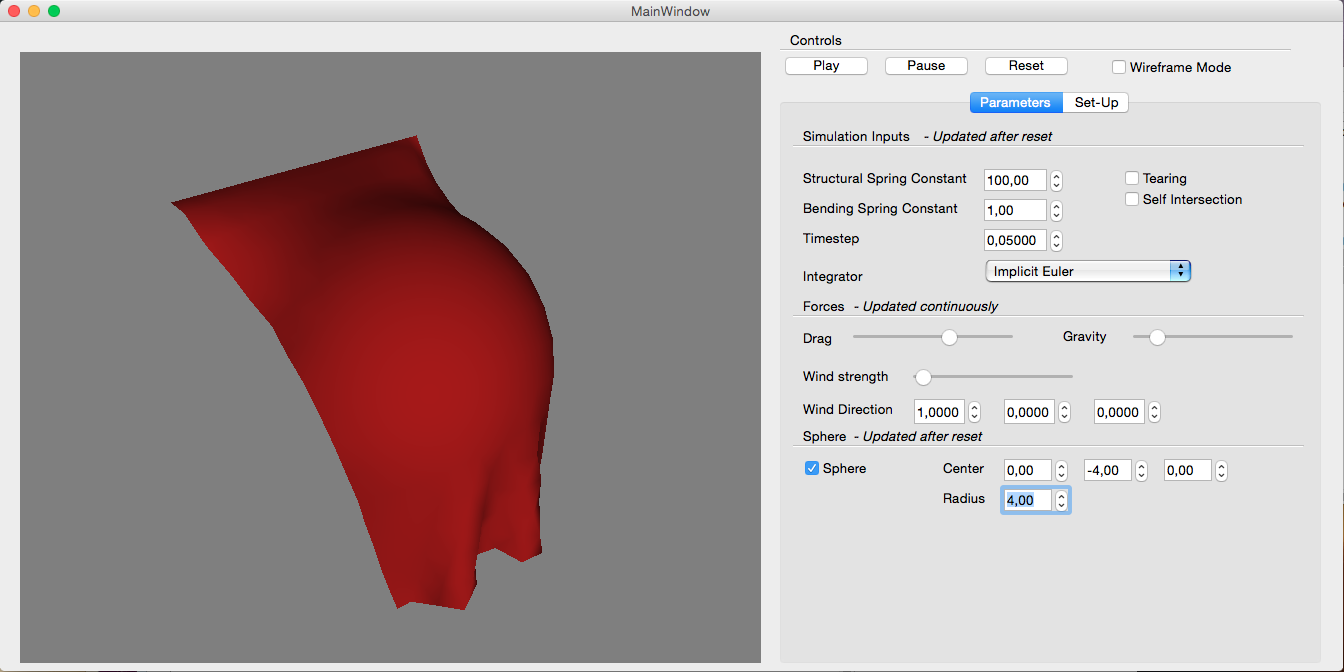
\includegraphics[width=4in,natwidth=366,natheight=166]{img/collision.png}
  \caption
   {Cloth resting on a sphere, simulated by the students software. Collision handling based on position based dynamics \citep{position_based_dyn}.}
 \label{collision}
\end{figure}

A similar self intersection handling algorithm was implemented, in the {\bf SelfIntersectionConstraint} class, based on the distance between non-connected particles. However, the student had no time left to test and debug this, and hence he is not sure that this is working correctly.


\ifx\isEmbedded\undefined
% References
\addcontentsline{toc}{section}{References}
\bibliographystyle{../ref/harvardnat}
\bibliography{../ref/master}
\pagebreak
\end{document}
\fi